%%%%%%%%%%%%%%%%%%%%%%%%%%%%%%%%%%%%%%%%%
% Large Colored Title Article
% LaTeX Template
% Version 1.1 (25/11/12)
%
% This template has been downloaded from:
% http://www.LaTeXTemplates.com
%
% Original author:
% Frits Wenneker (http://www.howtotex.com)
%
% Modified for use in class at Olin College of Engineering
%
% License:
% CC BY-NC-SA 3.0 (http://creativecommons.org/licenses/by-nc-sa/3.0/)
%
%%%%%%%%%%%%%%%%%%%%%%%%%%%%%%%%%%%%%%%%%

%----------------------------------------------------------------------------------------
%	PACKAGES AND OTHER DOCUMENT CONFIGURATIONS
%----------------------------------------------------------------------------------------

\documentclass[11pt, twocolumn]{article}
\usepackage[margin=1in]{geometry}
\usepackage{parskip}
\setlength{\parindent}{20pt}	%15pt normally

\usepackage[english]{babel} % English language/hyphenation
\usepackage{graphicx}
\usepackage[usenames,dvipsnames,svgnames,table]{xcolor} %usenames: 16 HTML base colors%dvipsnames: 64 more colors%svgnames: 150 colors%table: colors in tables

\usepackage{url} 	%allow url references in bibtex
\usepackage[colorlinks=true,urlcolor=DarkRed,linkcolor=DarkRed,citecolor=DarkRed]{hyperref}
%\href{mailto:jomm@olin.edu}{jomm at olin dot edu}


\usepackage[fleqn]{amsmath} % Math packages
\interdisplaylinepenalty=2500 %don't allow line breaks in the middle of multi-line equations

\usepackage[margin=1in]{geometry}

\usepackage[hang, normal,labelfont=bf,up,textfont=it,up]{caption} % Custom captions under/above floats in tables or figures
\usepackage{booktabs} % Horizontal rules in tables

\usepackage{sectsty} % Enables custom section titles
\allsectionsfont{\usefont{OT1}{phv}{b}{n}} % Change the font of all section commands

\usepackage{fancyhdr} % Needed to define custom headers/footers
\pagestyle{fancy} % Enables the custom headers/footers
\usepackage{lastpage} % Used to determine the number of pages in the document (for "Page X of Total")

% Headers - all currently empty
\lhead{}
\chead{}
\rhead{}

% Footers
%\lfoot{\footnotesize \today}
\cfoot{}
\rfoot{\footnotesize Page \thepage\ of \pageref{LastPage}} % "Page 1 of 2"

\renewcommand{\headrulewidth}{0.0pt} % No header rule
\renewcommand{\footrulewidth}{0.4pt} % Thin footer rule


%----------------------------------------------------------------------------------------
%	TITLE SECTION
%----------------------------------------------------------------------------------------

\usepackage{titling} % Allows custom title configuration

\newcommand{\HorRule}{\color{DarkGoldenrod} \rule{\linewidth}{1pt}} % Defines the gold horizontal rule around the title

\pretitle{\vspace{-30pt} \begin{flushleft} \HorRule \fontsize{20}{20} \usefont{OT1}{phv}{b}{n} \color{DarkRed} \selectfont} % Horizontal rule before the title

\title{Smart Lantern Workshop Pilot Report\\\vspace{.1in}{July 26-28, 2014, Orkolili, Tanzania}} % Your article title

\posttitle{\par\end{flushleft}\vskip 0.5em} % Whitespace under the title

\preauthor{\begin{flushleft}\large \lineskip 0.5em \usefont{OT1}{phv}{b}{sl} \color{DarkRed}} % Author font configuration

\author{Megan McCauley, Mika Ichiki-Welches, and Jose Oscar Mur-Miranda,\\} % Your name

\postauthor{\usefont{OT1}{phv}{m}{sl} \color{Black} % Configuration for the institution name
Olin College of Engineering % Your institution

\par\end{flushleft}\HorRule} % Horizontal rule after the title

%----------------------------------------------------------------------------------------
\date{} % Add a date here if you would like one to appear underneath the title block

\begin{document}

\maketitle % Print the title

\thispagestyle{fancy} % Enabling the custom headers/footers for the first page 

%----------------------------------------------------------------------------------------
%	ABSTRACT
%----------------------------------------------------------------------------------------

% The first character should be within \initial{} for a large character
%\noindent \textbf{This is the abstract text. It should summarize the main idea of the paper. Don't write abstracts that say ``I will analyze x and focus on y''. This is akin to saying ``In this paper, I will introduce a subject as mentioned in my title, analyze data relevant to it, and discuss some conclusions.'' The abstract is the juiciest possible content.}

%----------------------------------------------------------------------------------------
%	ARTICLE CONTENTS
%----------------------------------------------------------------------------------------

%-------------------------------Objectives
\section*{Objectives}
The International Development Innovation Network (IDIN) is an international consortium that fosters sustainable, local innovation through design, entrepreneurship and technology. A variety of hands-on workshops exposes network members to different technologies that can serve as design tools. The smart light workshop steps the participants through the construction of an LED lantern that incorporates a low-cost, programmable microcontroller.
The workshop is designed to:
\begin{itemize}
\item give participants basic electronic fabrication skills,
\item view electronic system design as being composed of interchangeable subsystems, and
\item introduce programmable feedback devices into their design thinking.
\end{itemize}
\includegraphics[width=.7\columnwidth]{the_lantern.jpg}

%-------------------------------Technology
\section*{Technology}
The smart light uses a PIC10F200 microcontroller to dim the perceived brightness of three LEDs using pulse-width modulation. The user can cycle through the different brightness levels by pushing a tactile switch. The circuit is powered by two AA batteries, and any container of the appropriate size may be used as an enclosure.
\includegraphics[width=\columnwidth]{lantern_push_button.jpg}

The microcontroller is used to regulate the power delivered to the LEDs. The power delivered from the AA batteries flows into the microcontroller, which then drives the LEDs directly connected to the output pins. Since LEDs can only be fully on or fully off, the microcontroller regulates the power delivered using pulse-width modulation.
%-------------------------------Stakeholders
\section*{Stakeholders}
We have identified four distinct stakeholders for this pilot. The first stakeholders are students at the Orkolili Secondary School, which can then be further subdivided according to their role in the workshop. These four subgroups of students are: workshop teachers, workshop participants, workshop observers, and the remaining students with whom we had no interaction. The second stakeholder is Mama Mcha, as the founder and manager of the school. The third stakeholders are the members of the IDDS/IDIN community. The fourth group of stakeholders is the teachers at the school.

Our first stakeholders are those who are directly prospering from the teaching of the smart light workshop: \textbf{the students}. The first subset of student stakeholders was the student teachers. The student teachers played the unique part of being both student participants—on day one, when we were the instructors—and teachers—on day two, when they were in charge. We turned over complete instruction of the workshop to them and they were responsible for teaching another subset of student learners. Another subset of the student stakeholders that should be taken into account were the student observers who surrounded our work tables on both days. Although they did not get any official hands-on experience with the tools or materials, they still gained knowledge and inspiration from watching and listening to the workshop as the other students completed their lanterns. Now, all of the students, from the learners to the teachers to the observers, have the opportunity to become designers, explorers, and innovators. For completeness, there is fourth group of student stakeholders composed of those with which we had no contact. Although we have no evidence, it is reasonable to assume that some of these students will benefit indirectly from the workshop.

\textbf{Mama Mcha}, the founder and manager of the Orkolili Secondary School, was our second stakeholder. Mama Mcha is driven by her passion for teaching and she encourages this passion as the essential driver for her students’ learning. Her values define the context and experiences of her students. In particular, she aims to develop creativity and responsibility in her students. Because of this, she also develops hands-on fabrication skills as part of her curriculum. In particular, she is responsible for getting her students excited about the prospect of learning engineering skills by promoting curiosity and challenging their skills, while at the same time instilling self-confidence. Mama Mcha also challenges gender stereotypes by allowing her female students to wear pants on the weekend and encouraging them to participate in the same subjects and activities as her male students.

Our final stakeholders are the \textbf{International Development Design Summit (IDDS)} and the International Development Innovation Network (IDIN), which are both funded by USAID and a part of the USAID Development Lab. Our workshop was facilitated by the IDDS 2014 in Arusha, Tanzania. Two IDDS project teams had been working on this site before we arrived. More importantly, the outcome of this workshop in meant to increase the range of IDDS projects in the long run by giving us the confidence that microcontroller technology is appropriate in developing context and can be used effectively to alleviate poverty issues.

We did not have the opportunity to interact with any \textbf{school teachers}, but there several ways in which they can be both impacted by and have an effect on the workshop. Given their importance in the context, we have included them as an explicit stakeholder.

%-------------------------------Site
\section*{Site}
The characteristics of this site were a large contributor to the success of the workshop. As a result of Mama Mcha’s values and goals for the school, the Orkolili secondary school students were ideally suited to benefit from the smart light workshop. The school has students from 6th to 12th grades (as an approximate equivalency in the USA system). The age of students ranges from around 12 to 18. Our participants where 11th or 12th grade students with ages around 16. Even though it is not a boarding school, many students do not commute to their homes daily.

The relatively advanced facilities of the school support a hands-on curriculum. For example, all students, regardless of gender, learn how to sew and are required to sew some of their own clothing. The school also has a computer lab that runs on both Windows and Ubuntu operating systems. All students take high level science classes, including biology, physics, and chemistry, where they complete hands-on labs.

%-------------------------------Methods
\section*{Methods}
In order to devise appropriate methods of teaching and building the lanterns, we utilized bodystorming. Bodystorming is a user-centered approach where the participants get up and use physical movements in order to better understand concepts. In our case, bodystorming was essential for demonstrating the proper way to solder. We had the students act out each of the components involved in soldering: the soldering iron, wire, solder, and each electrical component. This interactive demonstration was particularly useful because of the complexities involved in describing soldering and the small scale that it would have had to be demonstrated on with the actual components.
\includegraphics[width=\columnwidth]{bodystorming.jpg}

Another technique that we used to assist in the building of the lanterns involved using wood blocks and sticky tack to assist in the process of soldering. The wood blocks were initially used to protect the tables from being burnt by the hot tip of the soldering iron. The sticky tack idea was generated last year during the same smart light workshop at IDDS 2013 in Zambia by another research student. The sticky tack holds down the components and frees up your hands to perform the actual soldering process. The concept behind this is that soldering typically requires at least three hands: one to hold the soldering iron, one to hold the solder, and one to keep the components flat on the work surface. There are many complicated and expensive devices to help with this, marketing themselves as “Third Hand” kits and the “Helping Hand.” However, with the combination of sticky tack and the wood block, we have created a simple, low-cost solution to this problem.
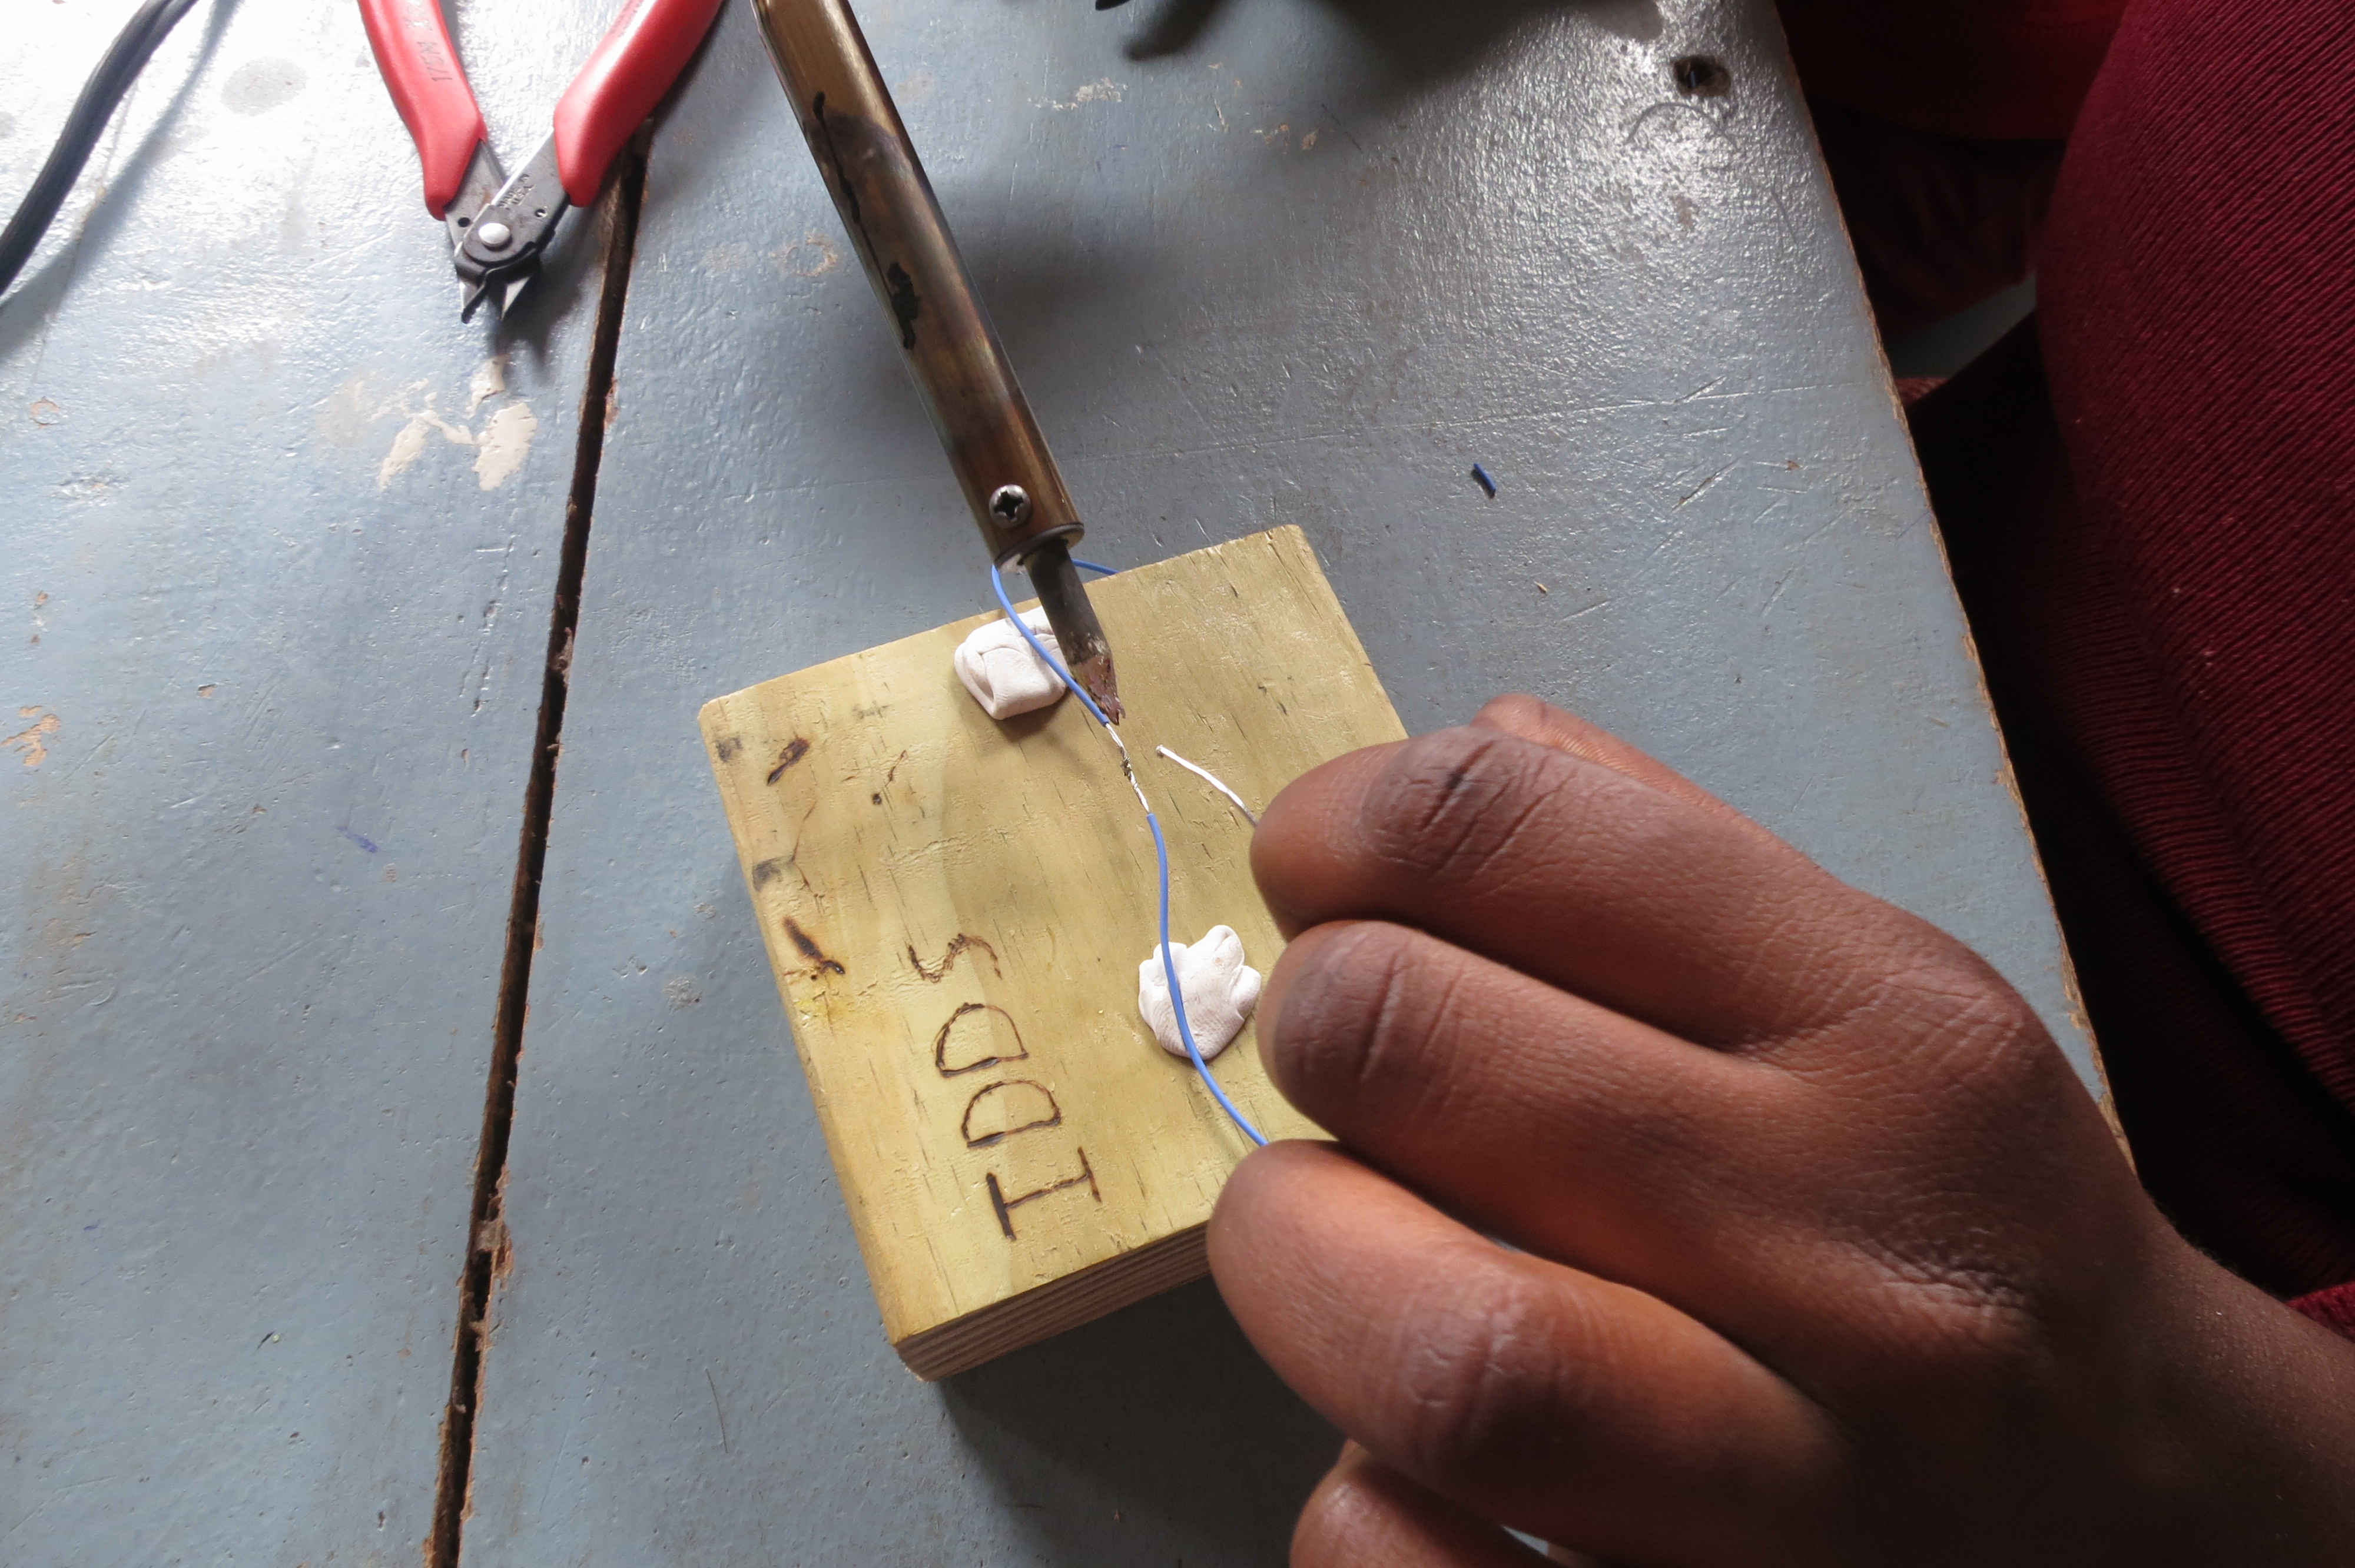
\includegraphics[width=\columnwidth]{wood_block_soldering.jpg}

We utilized peer teaching by having the students turn around and become the teachers.  On day one, we taught the workshop to eight students with the explicit expectation that they would teach the workshop the next day. Of those eight students, four became student teachers on the next day. The ability to take the knowledge that they learned the day before and relay it to their peers is generally an equalizing and empowering experience for students. Not only had they built their own smart light, but they owned the knowledge and made sure that one of their classmates was able to do the same. This system that we set into place allows for ease of replication of the workshop and a sense of sustainability because the teachers are students who attend the Orkolili Secondary School.
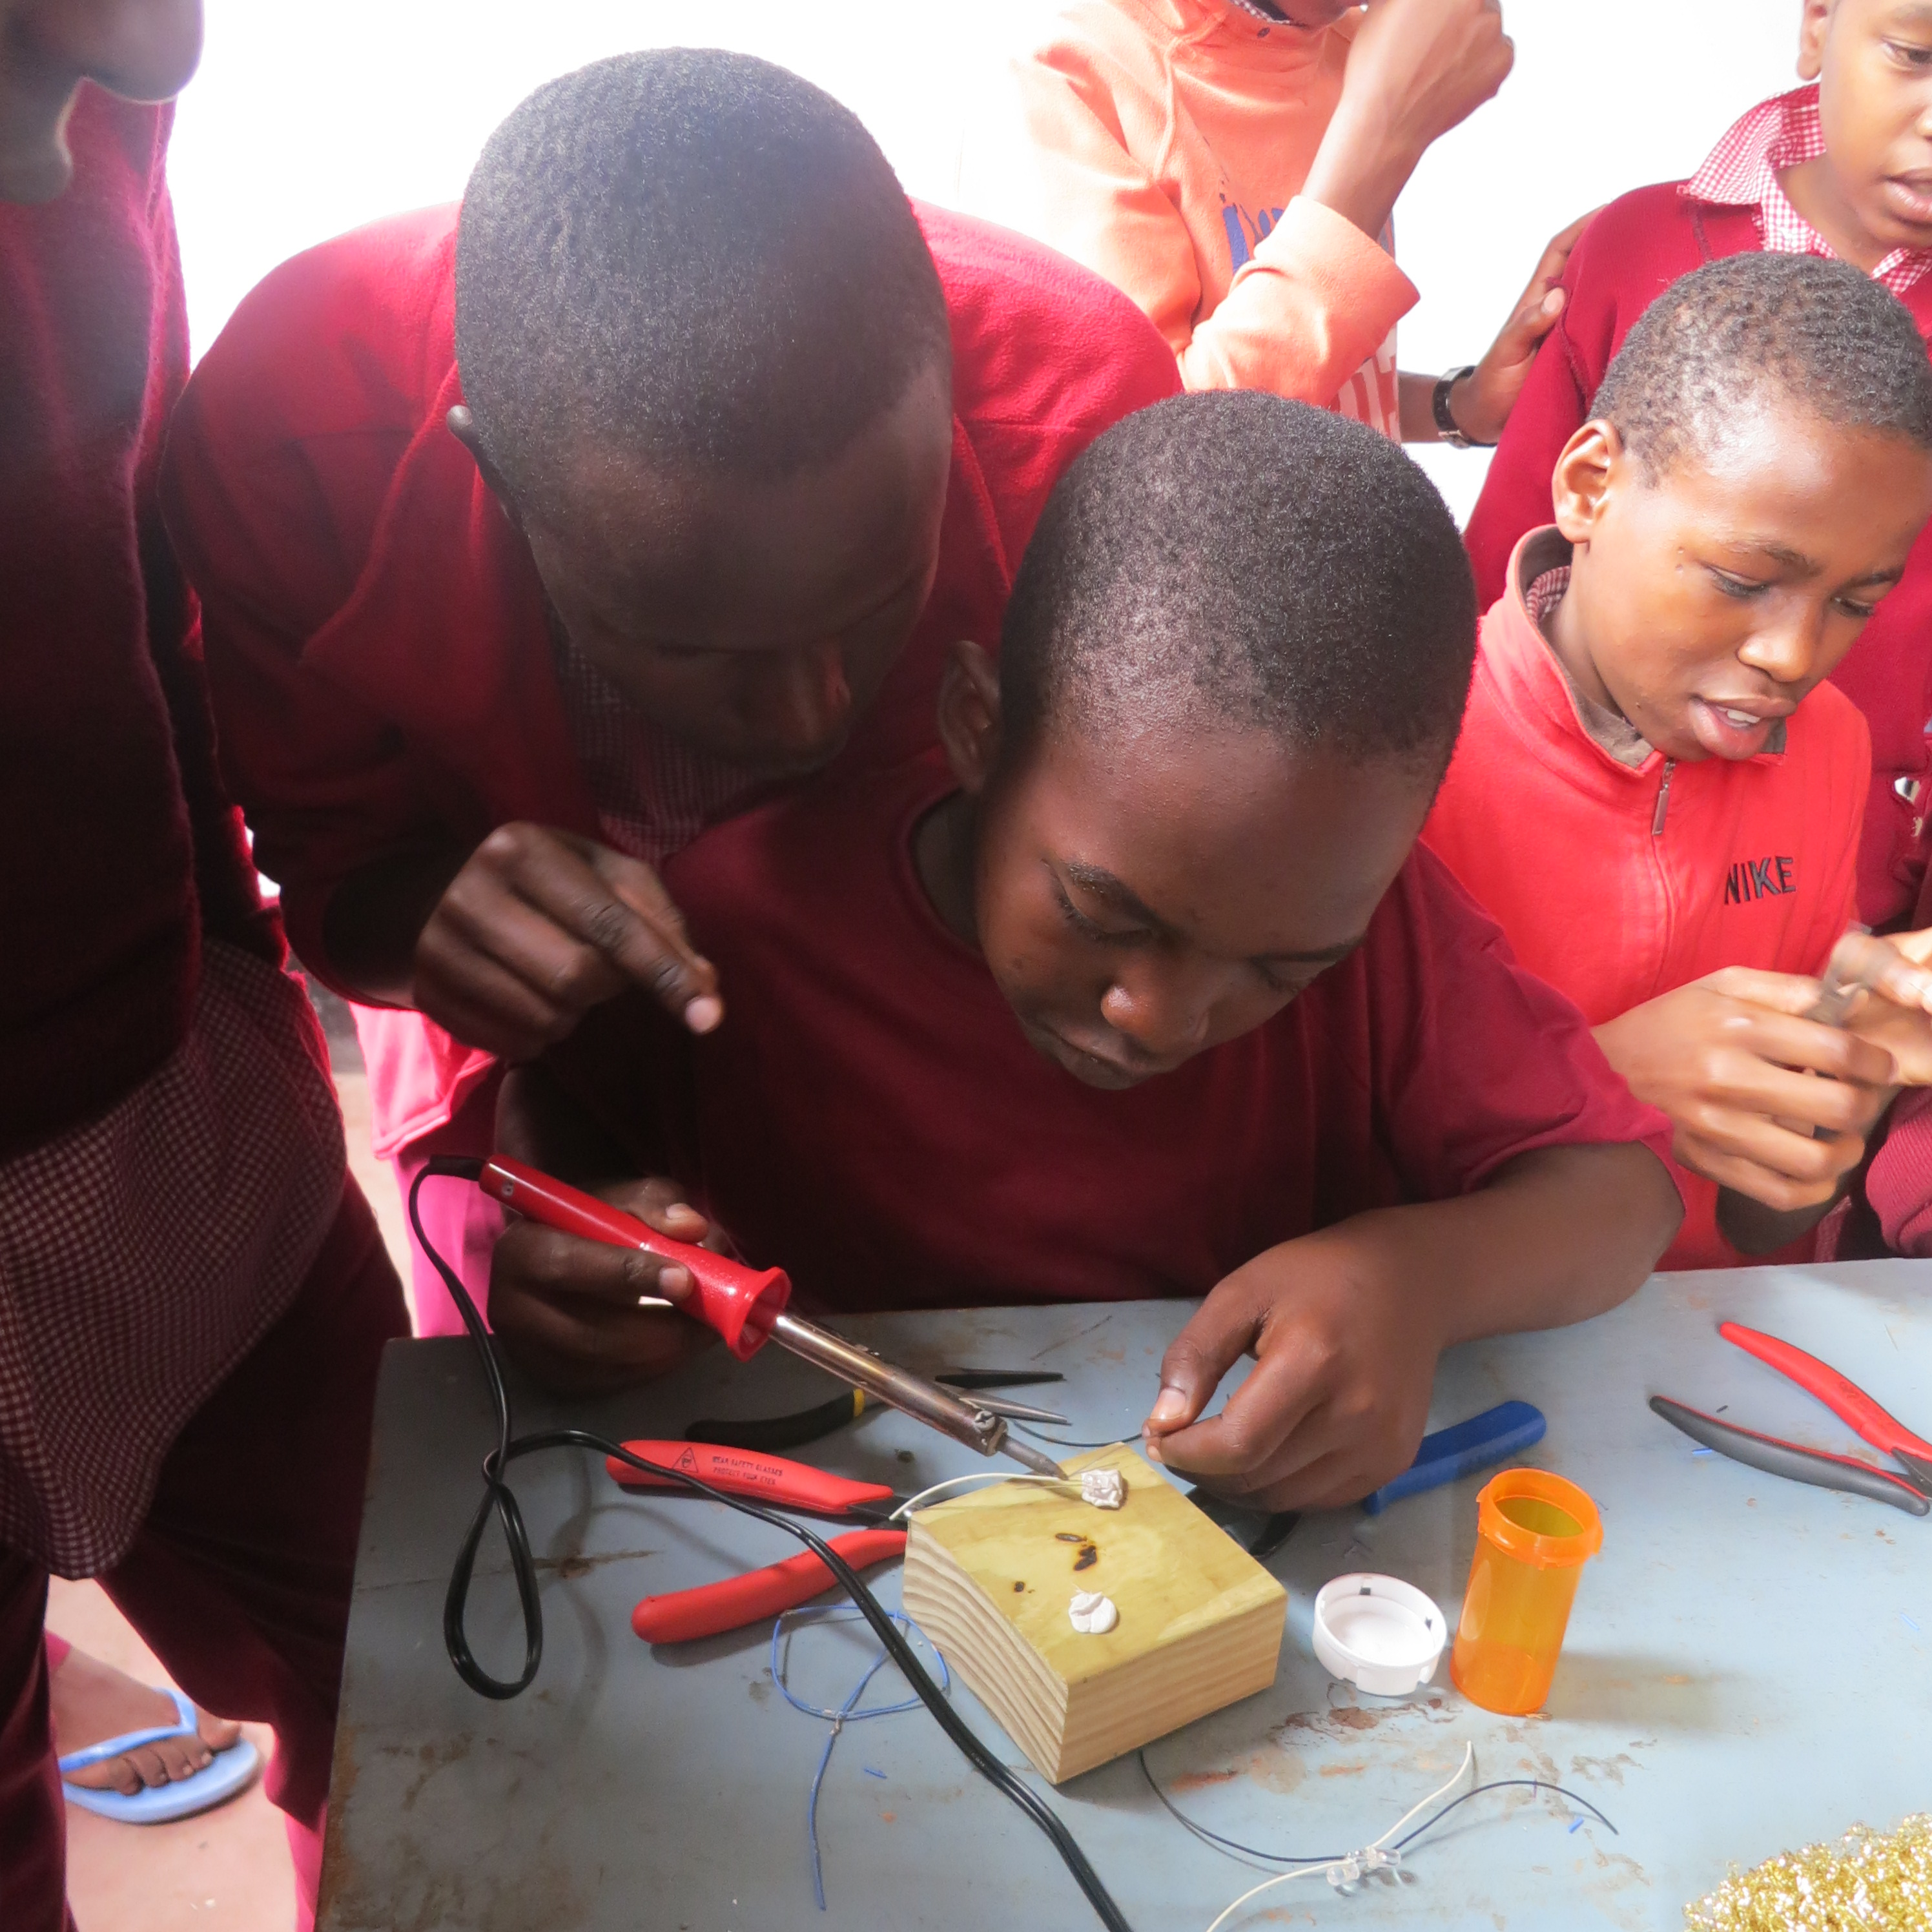
\includegraphics[width=\columnwidth]{teachers.jpg}\\
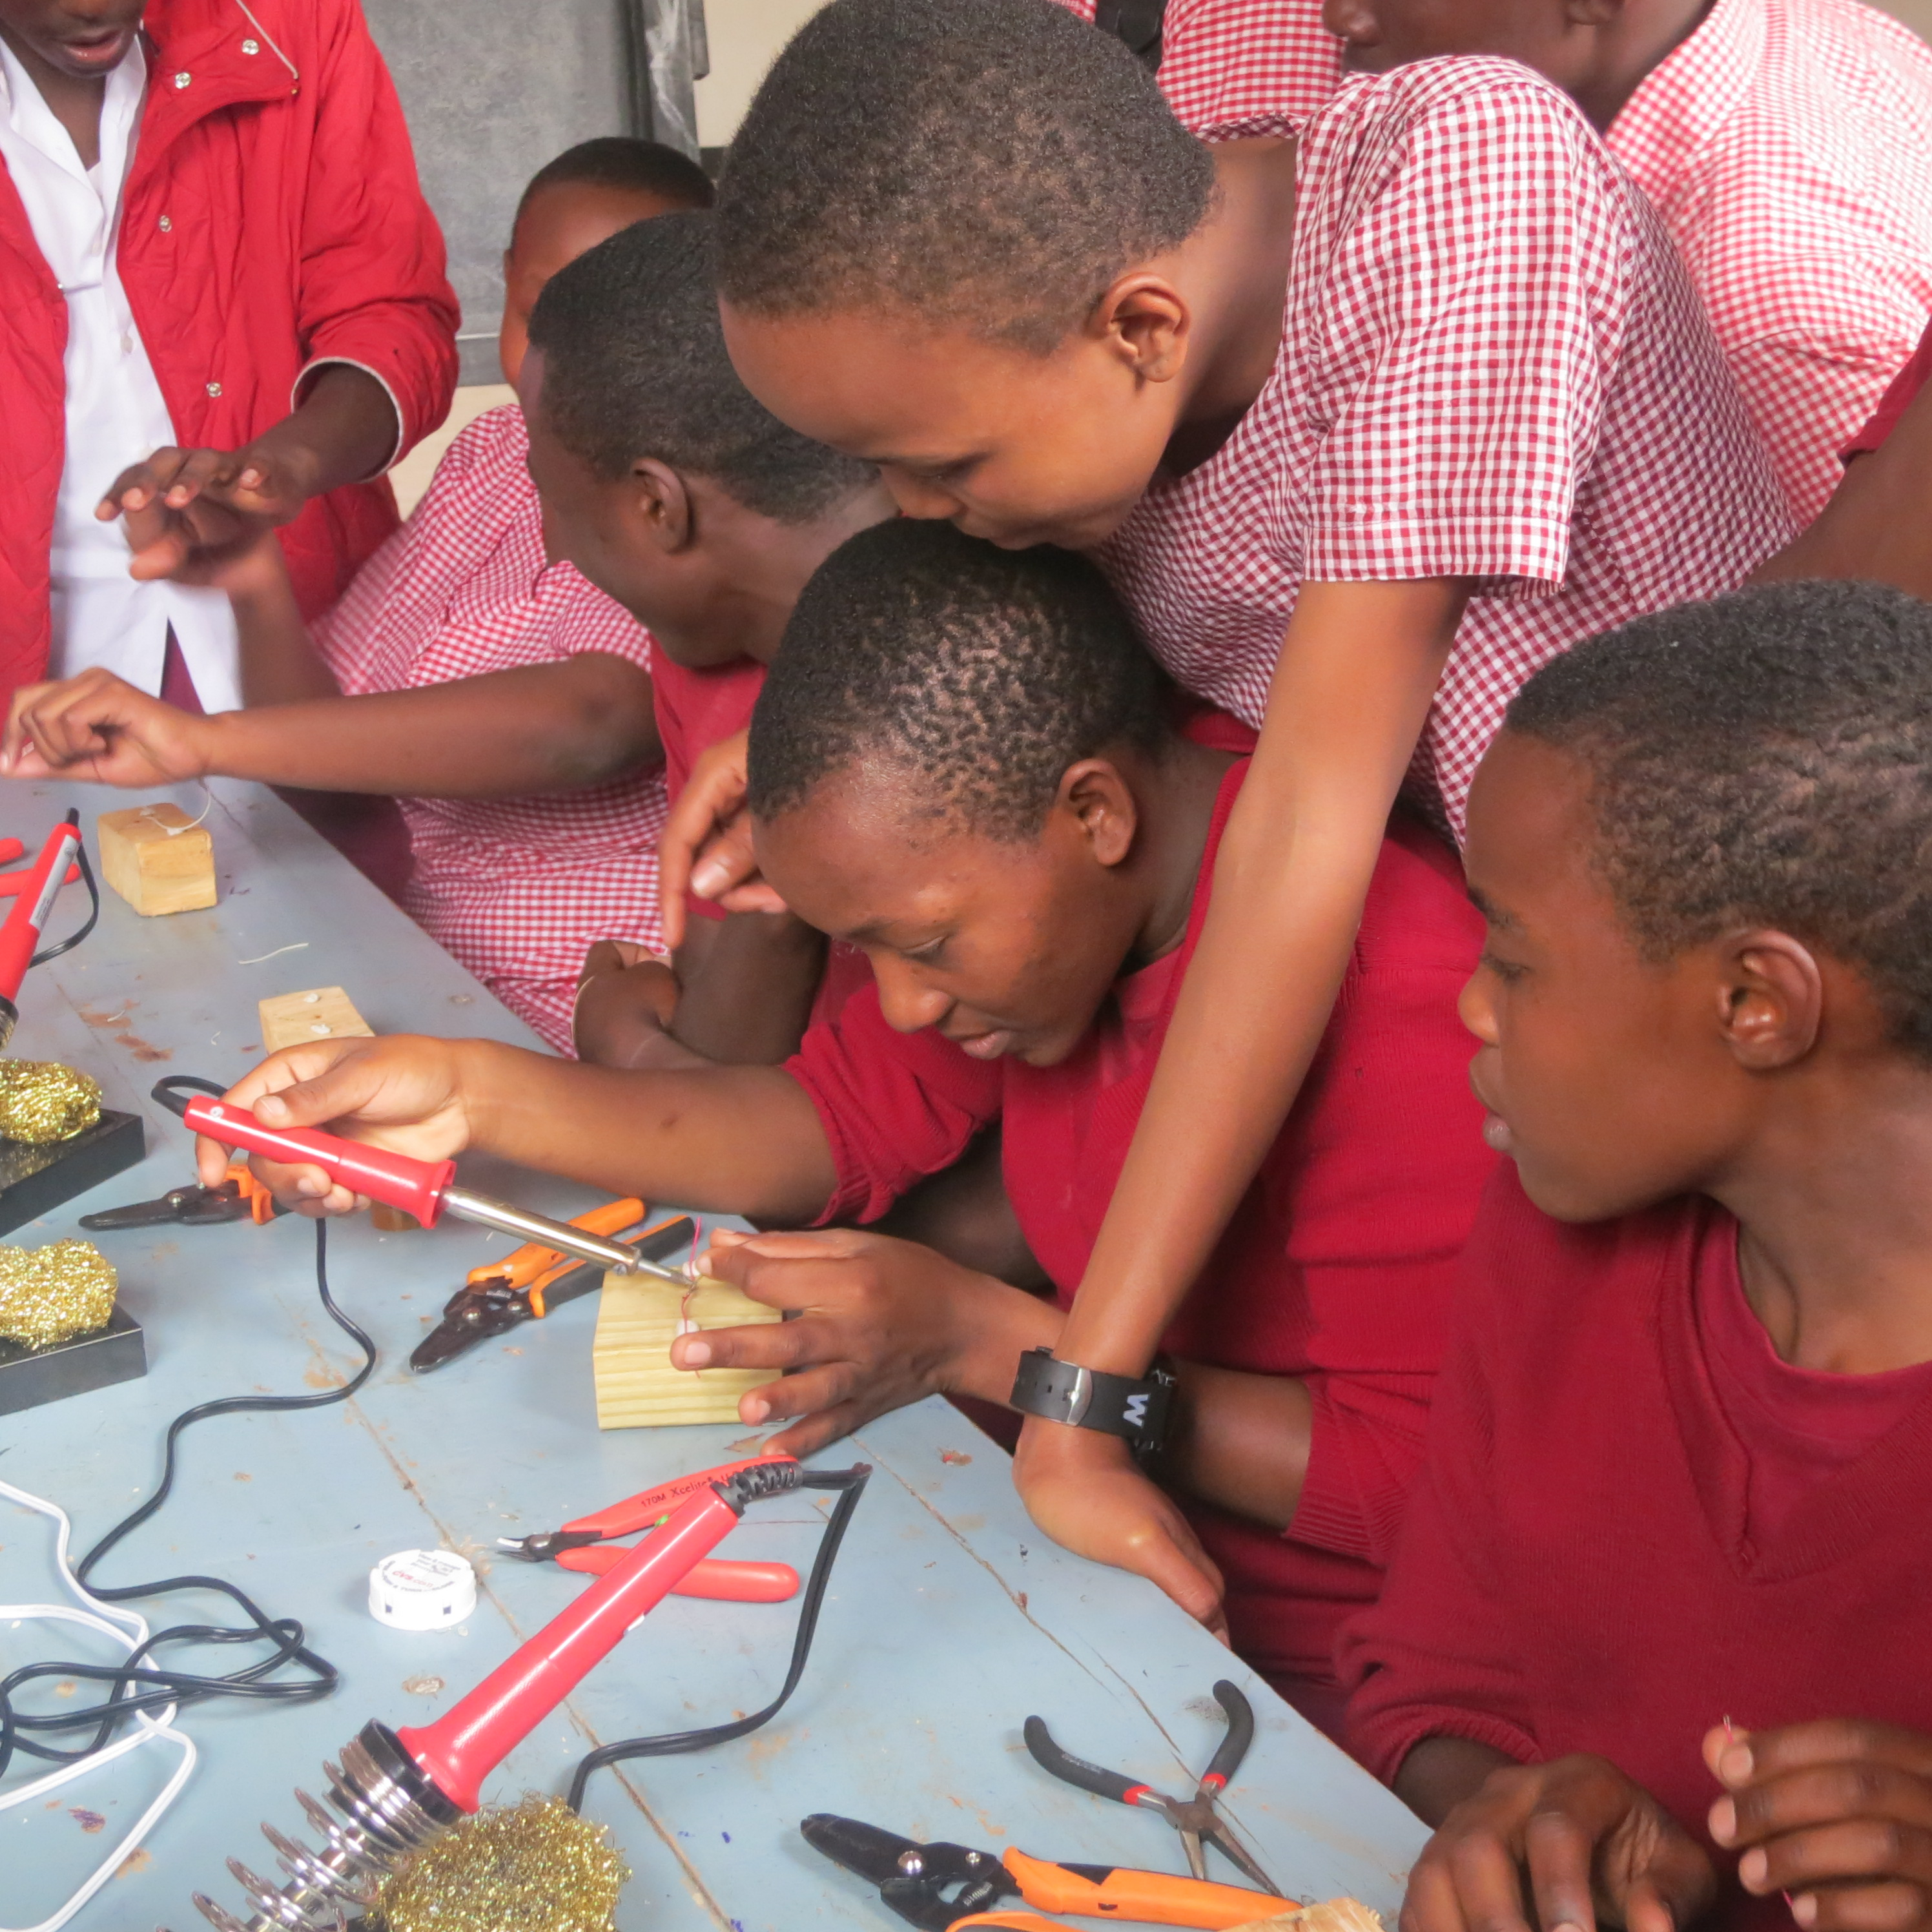
\includegraphics[width=\columnwidth]{more_teachers.jpg}

We also enabled exploration on the third day we were at the school, by providing students with uninhibited access to the soldering irons. This was an opportunity for exploration and innovation. We brought the soldering irons that they had been working with and left all of our supplies readily available. Throughout the day, students brought their broken flashlights from home to fix. Some of them were even able to determine what was wrong with them and fix them on their own, and with each other’s help. We also had cases of the students innovating through creation of different lanterns made my combing parts of their own broken lanterns with the LEDs and microcontrollers that we brought as part of the smart light workshop. The idea behind this is that the students would be able to see the value in their own designs and see themselves as designers.
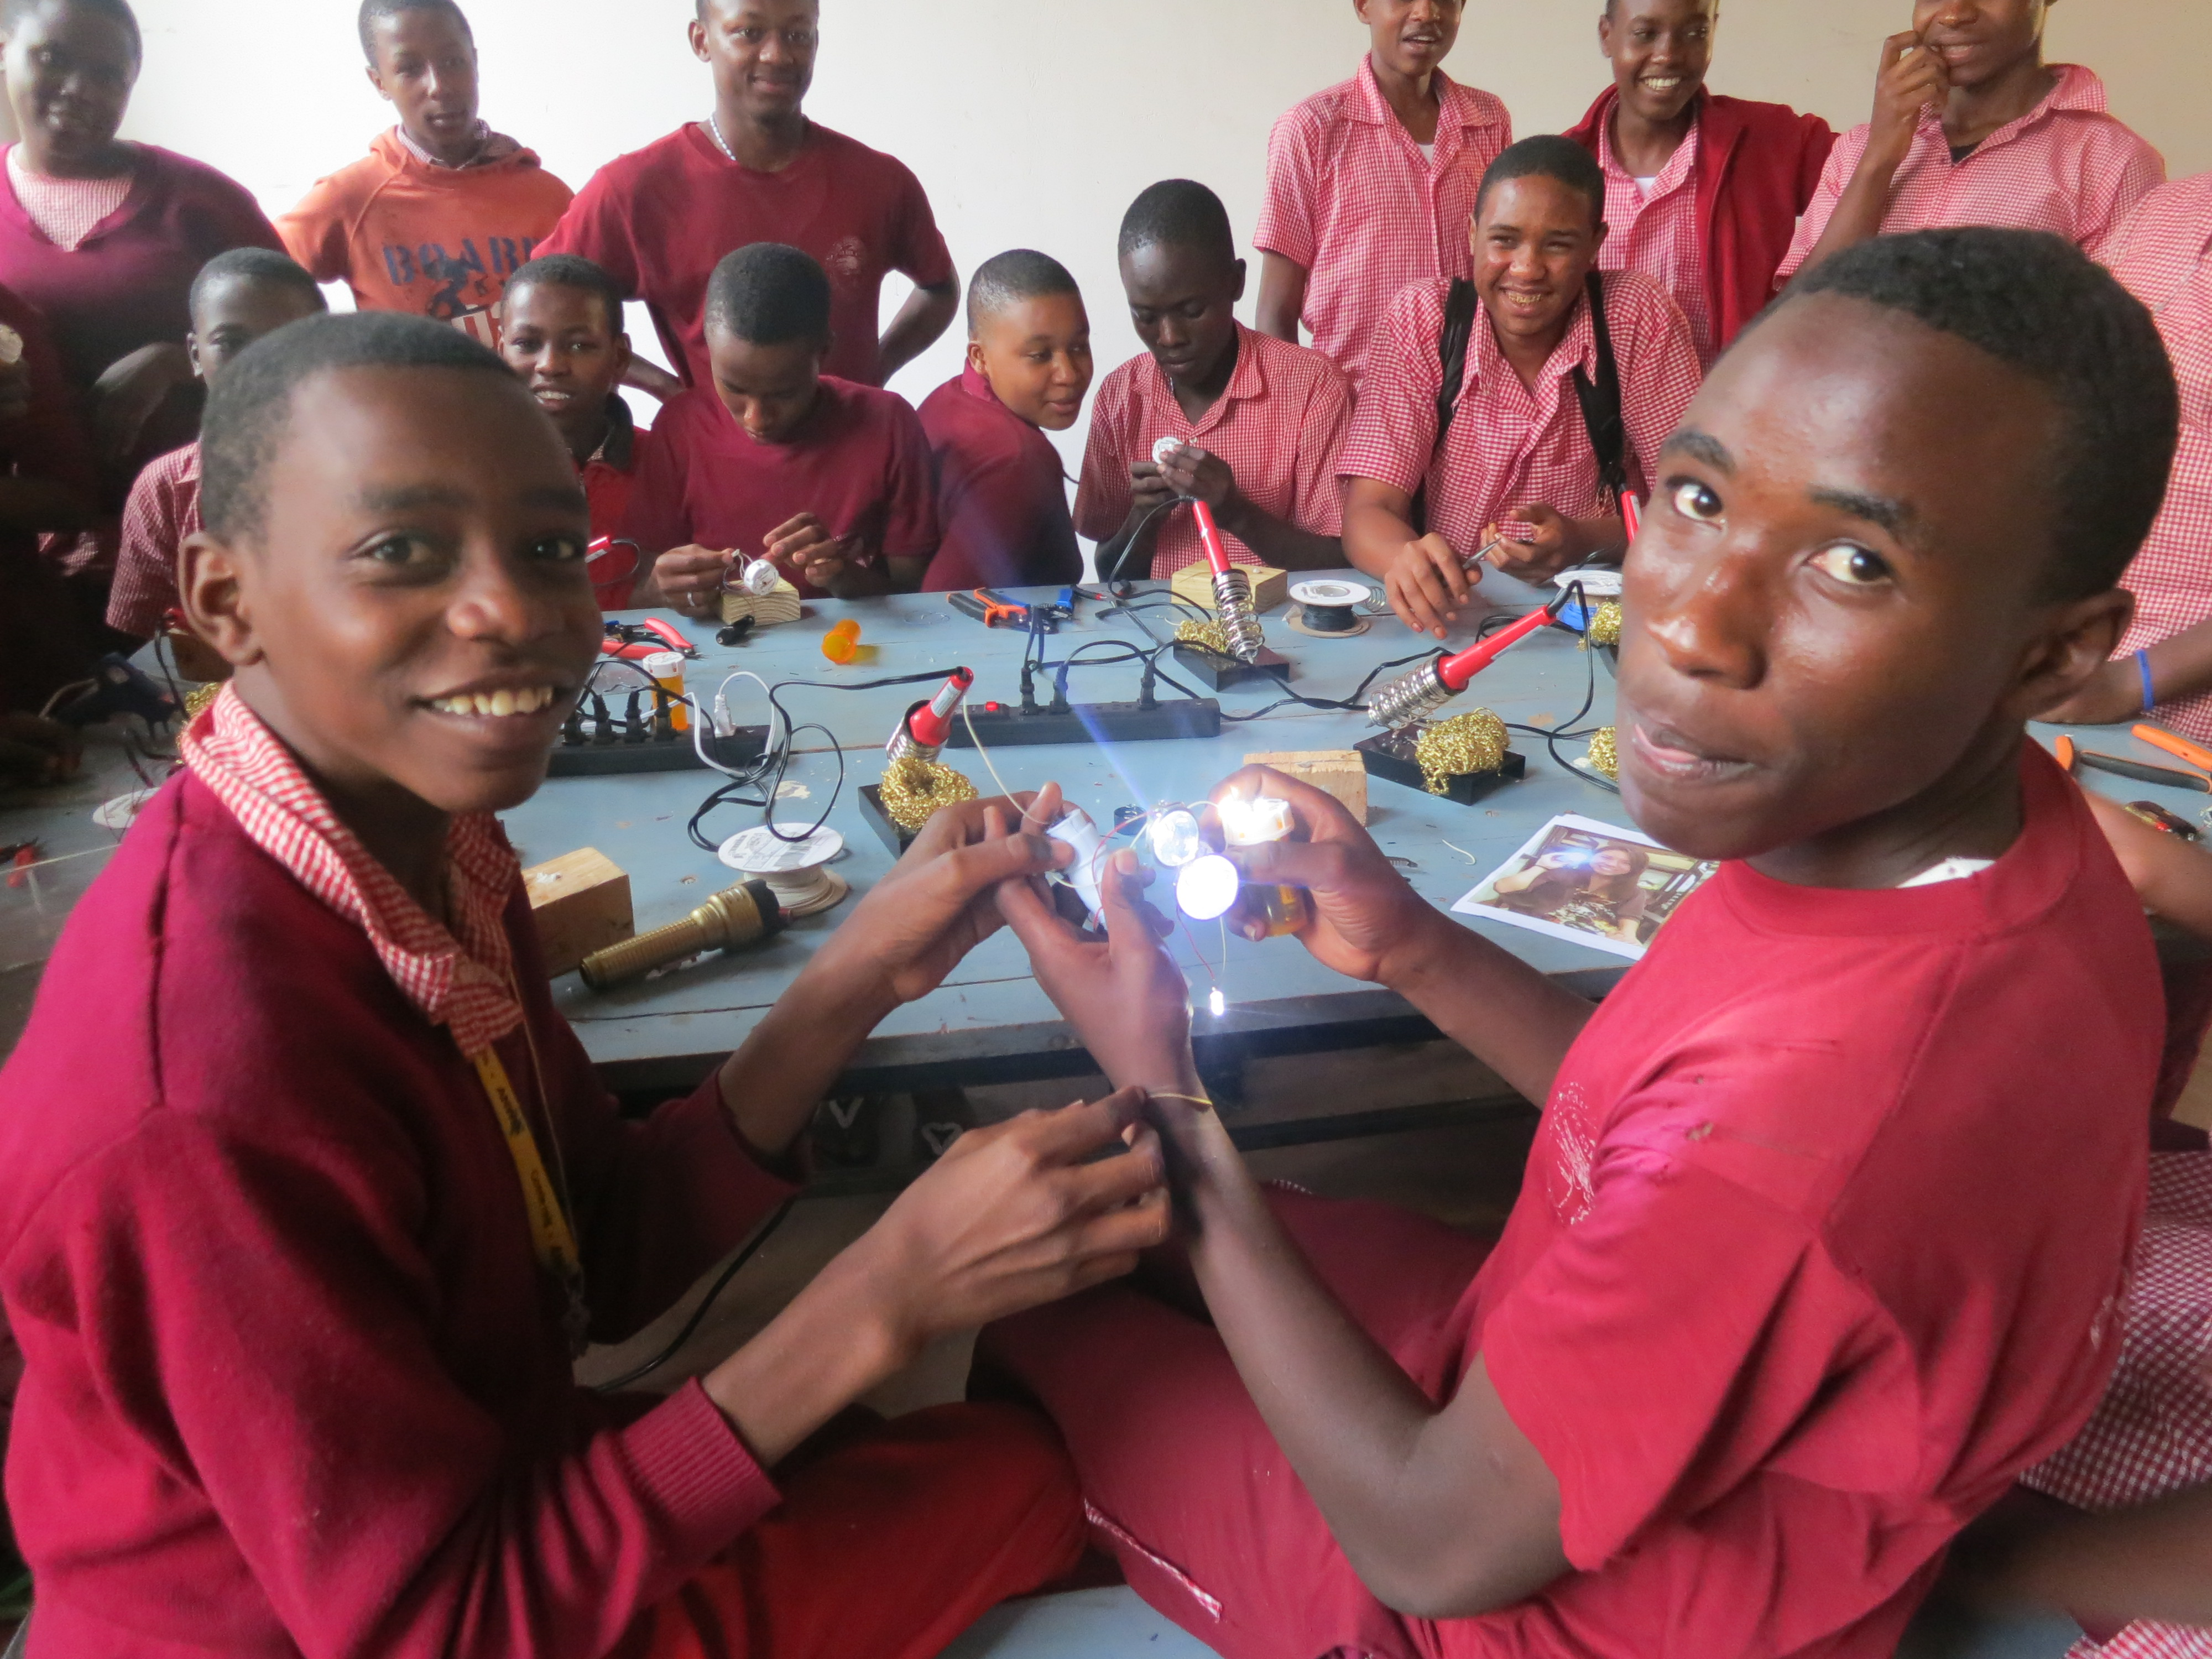
\includegraphics[width=\columnwidth]{innovation_students.jpg}\\
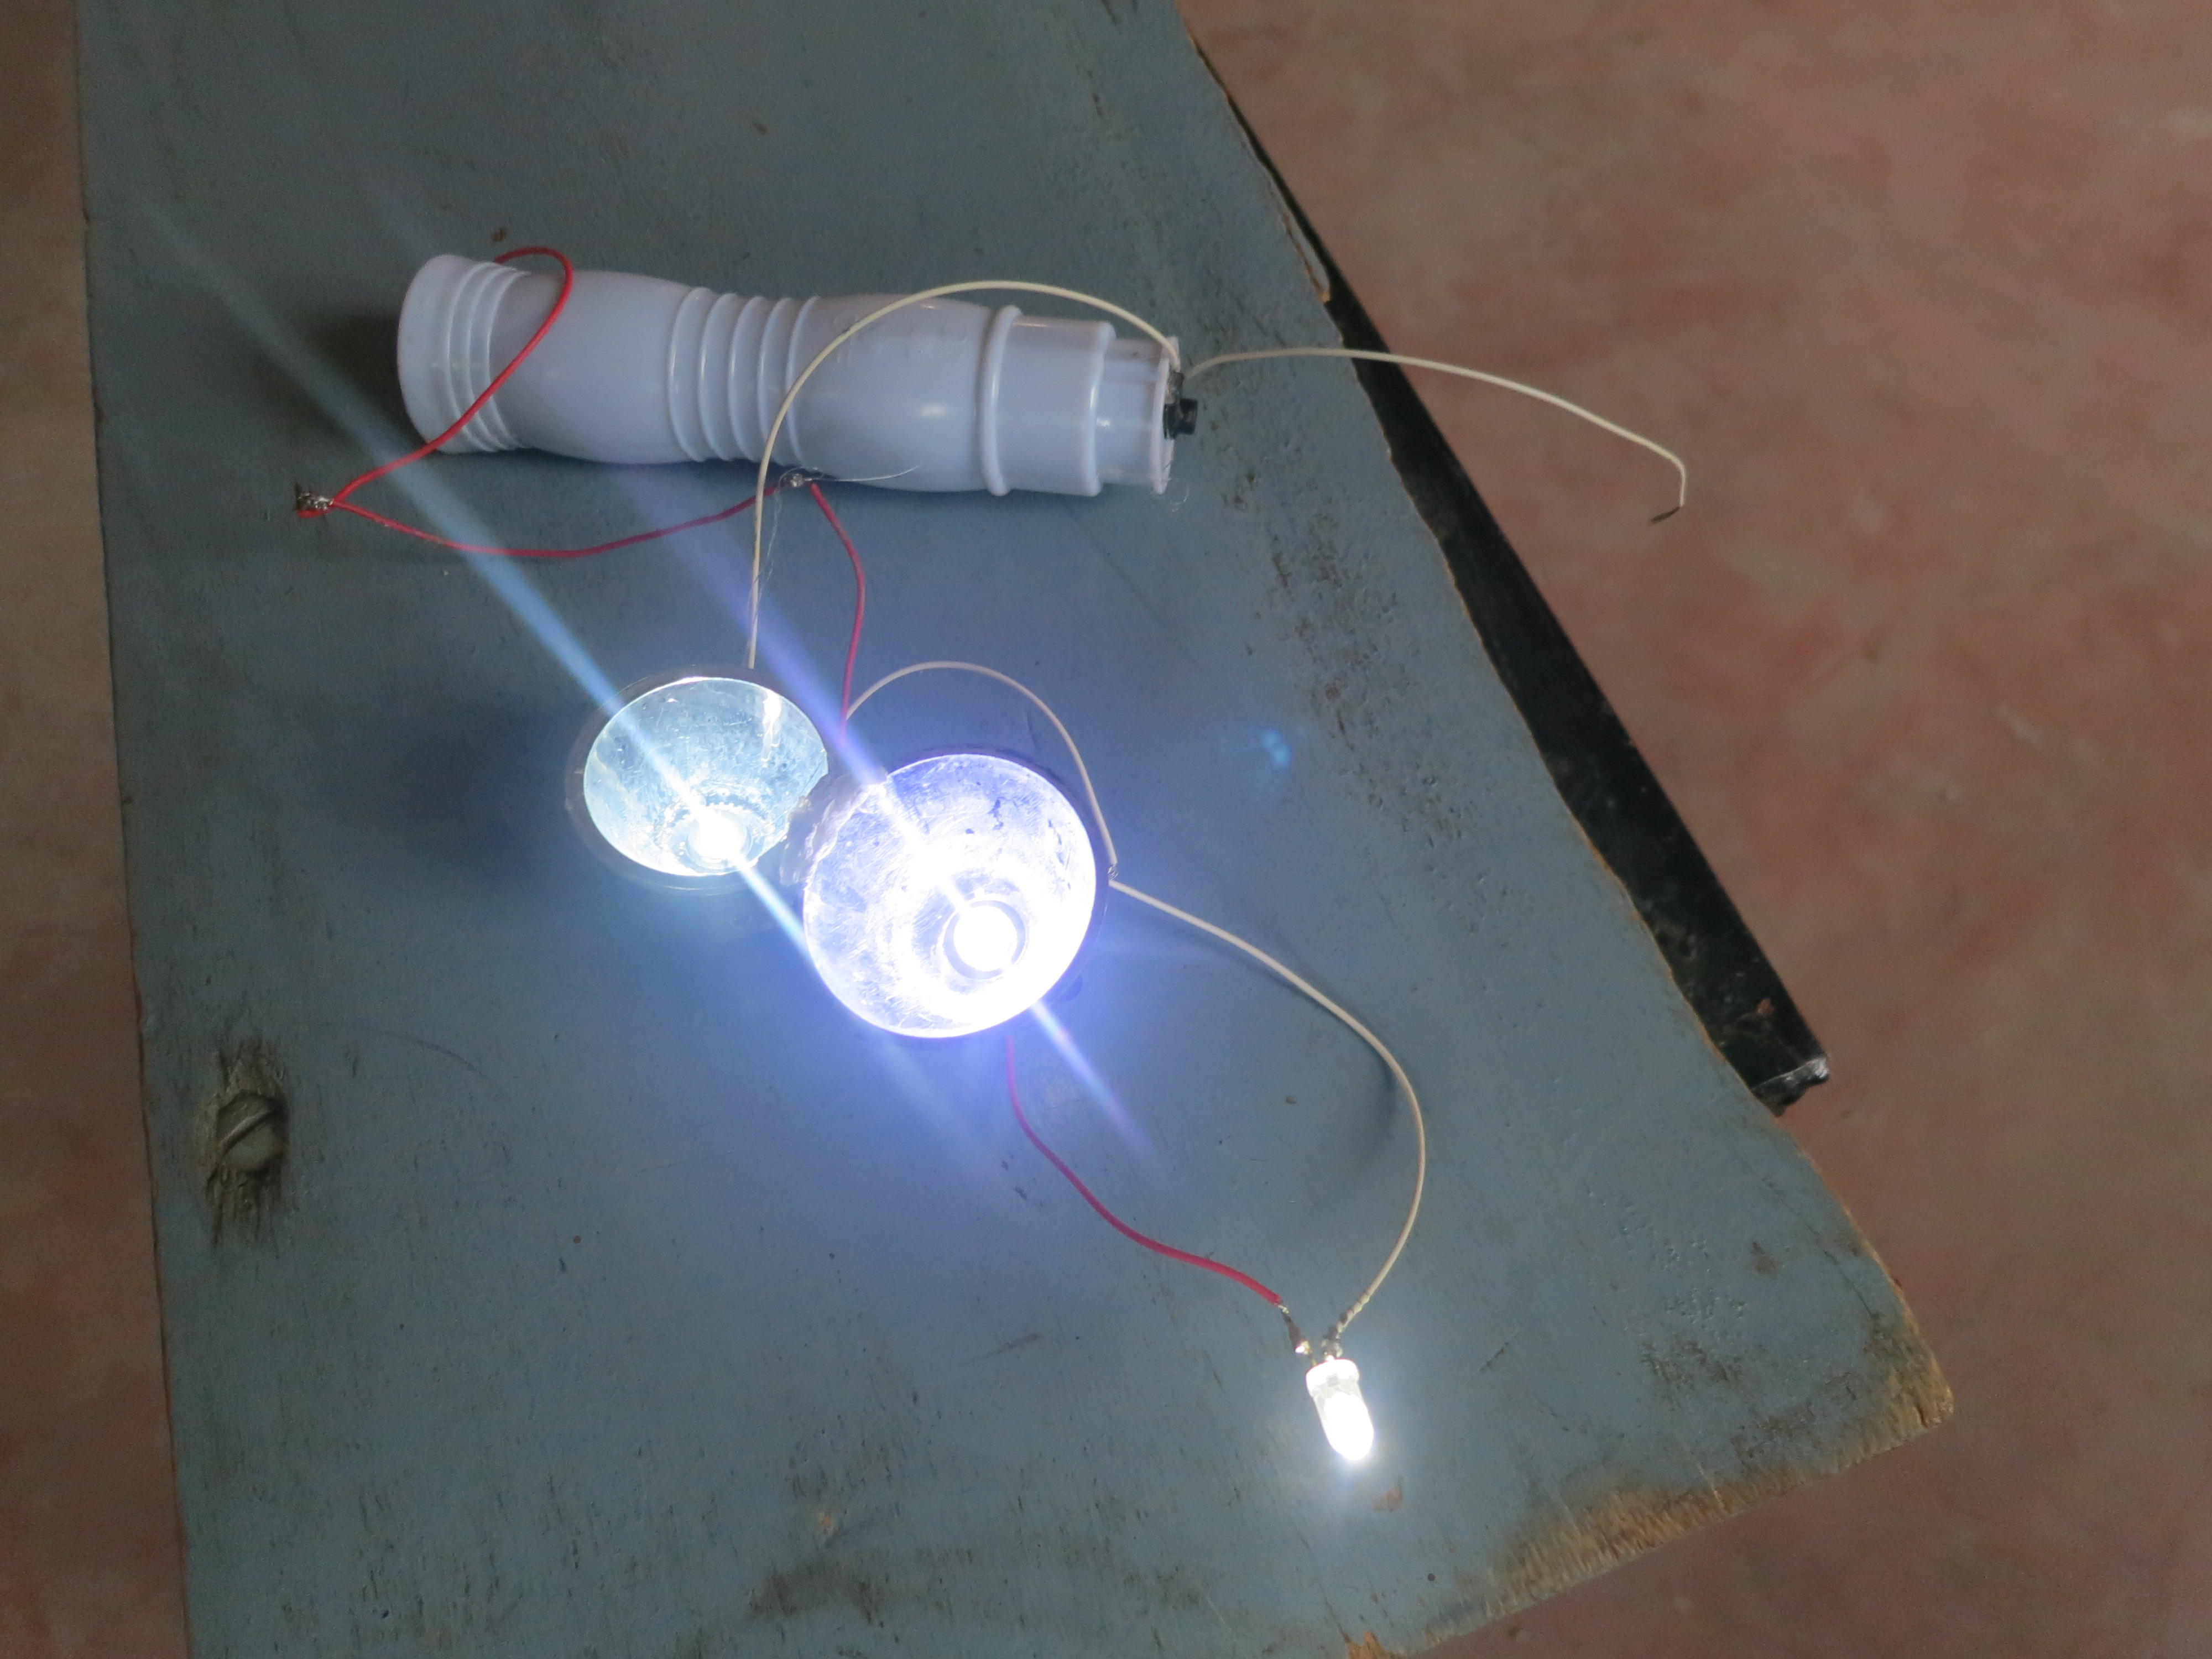
\includegraphics[width=\columnwidth]{innovation_lantern.jpg}

%-------------------------------Results
\section*{Results}
The first goal, fabrication skills, was met with absolute success. Bodystorming was essential in giving participants a clear sense of the how to solder in a humorous context that made it fun and memorable. Additionally, the soldering technique using wood block and sticky tack substantially increased the quality and reliability of solder joints from absolute beginners. Furthermore, student teachers became so proficient at soldering and fabrication that they were to focus their attention on the system itself. This focus allowed the student teachers to effectively troubleshoot the problems they saw.

Mastery of fabrication was essential to enable a subset of students to understand the system as a modular set of interchangeable blocks. Both student participants, and to a much clearer extent, student teachers, were able to diagnose fabrication problems by designing tests that isolated the different subsystems. In this way, they were able to differentiate a burned out LED from an incorrect solder connection or an unresponsive microcontroller. Since the physical phenomena in electrical engineering is not visible (i.e. voltage and current), what happens inside the system can only be determined indirectly by relying on visible effects. Thus, the student's ability to troubleshoot suggests they had confidence in abstract models of the system.

Furthermore, the creation of mental models was also evident when some participants were able to identify the equivalent subsystems in their own lanterns. The lanterns where visually very different, but the participants were able to fix them using their knowledge of the smart light and their fabrication skills.

At the extreme, in at least two occasions, participants were able to combine parts from their own lanterns with parts from our workshop to create new designs that were different from both the design of the smart light and their own lantern. This is the ultimate goal of the program, to enable local creation of new systems. Our future expectation is that the participants are able to create new designs that address local needs in their lives or their communities.\ \\
\ \\
Since we have not found an effective way for participants to reprogram the microcontroller, we have no evidence at this point for our third goal, the incorporation of feedback and programmability in their design thinking. While participants were told that the microcontrollers were programmed and that their behavior could be changed, the workshop itself does not allow them to do this. We hope to either create additional workshops, or expand this workshop so that participants are able to change the programming in order to achieve different behavior according to their designs.

%----------------------------------------------------------------------------------------
%	HOW TO FIGURES
%----------------------------------------------------------------------------------------

%Make you graphics big! In order to let a figure extend the two columns, add an asterisk (*) after figure like this:
%\begin{verbatim*}
%\begin{figure*}
%...
%\end{figure*}
%\end{verbatim*}

%Figures and tables should always be referenced within the text, as in the case of Figures~\ref{fig:myfigure} and~\ref{fig:myfigure2} and Table~\ref{tab:mytable}.

%\begin{figure*}
%\centering 
%\includegraphics[width=\textwidth]{Populati2012.pdf}\caption{\label{fig:myfigure}As much as possible, the graph should speak by itself. However, you should write a caption that captures a more nuanced analysis of the dataset. The source citation should be in the caption directly. {\tt Data: World Bank World Development Indicators~\cite{wdi}. Source code for figure: \url{https://github.com/jabb1123/RADical/blob/master/Oscar/population_plot.py}}} 
%\end{figure*}

%----------------------------------------------------------------------------------------
%	REFERENCE LIST
%----------------------------------------------------------------------------------------

%References should be done like this~\cite{collier2001}.

%\begin{thebibliography}{9}
%
%\bibitem{collier2001}
%Collier, Paul and Dollar, David, (2001), Can the World Cut Poverty in Half? How Policy Reform and Effective Aid Can Meet International Development Goals, World Development, 29, issue 11, p. 1787-1802.
%
%\bibitem{wdi}
%World Bank. World Development Indicators (WDI) online database. Washington, DC. \url{http://data.worldbank.org/data-catalog/world-development-indicators}. Data retrieved September 24, 2014.
%
%\end{thebibliography}

%----------------------------------------------------------------------------------------

\end{document}